\documentclass[12pt]{beamer}
\usepackage{xspace}
\usepackage{listings}
\lstset{
  texcl=true,
  basicstyle=\small,
  numbers=left,
  numberstyle=\tiny,
  frame=single,
  columns=fullflexible
}
\usepackage{graphicx}
\newcommand{\mint}{{\sffamily MINT}\xspace}

\title{The \mint neural network library}
\author[S Ghirlanda]{Stefano Ghirlanda}
\subtitle{A quick introduction}
\date{\today}

\begin{document}

\begin{frame}
  \titlepage
\end{frame}

\begin{frame}{Problems of existing simulation software}
  \begin{itemize}
  \item Engineering view of neural networks
  \item Not general enough
  \item Too low level for my (our) purpose
  \item Makes things complicated
  \item Costs money
  \end{itemize}
\end{frame}

\begin{frame}[fragile]{Data structures: Nodes}

\begin{lstlisting}
mint_nodes n;

/* create 10 nodes with 1 state variable each */ 
n = mint_nodes_new( 10, 1 ); 

n[0][i]; /* input to node i */
n[1][i]; /* output of node i */
n[2][i]; /* current value of 1st state variable of node i */

for( i=0; i<mint_nodes_size(n); i++ )
  n[0][i] = mint_random();

mint_nodes_update( n );

\end{lstlisting}

\end{frame}

\begin{frame}[fragile]{Architecture files}

\begin{lstlisting}
nodes brain
size 10 logistic 0.1 1 
\end{lstlisting}
  \begin{center}
  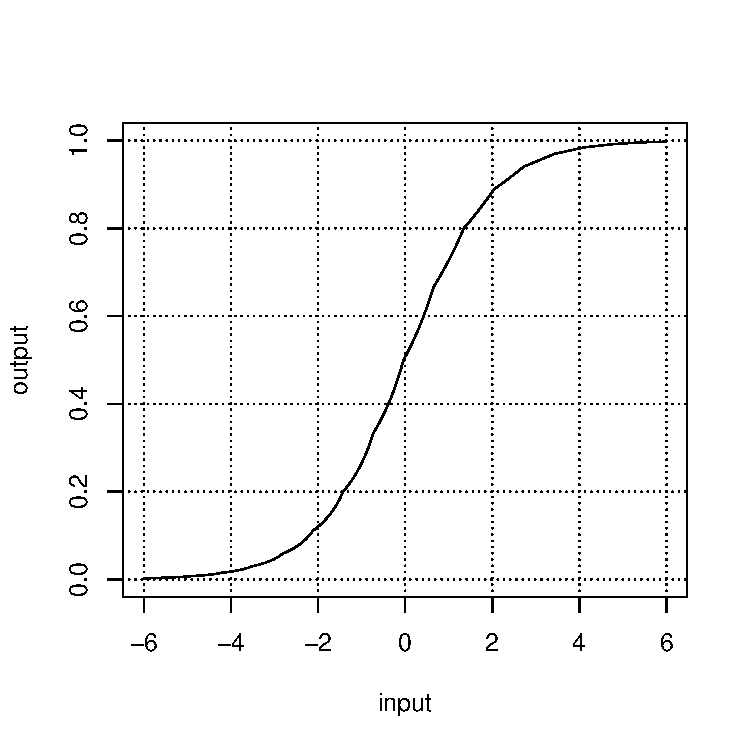
\includegraphics[width=.6\textwidth]{%
    ../../example/logistic/logistic}    
  \end{center}
\end{frame}

\begin{frame}[fragile,fragile]
  \frametitle{Data structures: Weights}
  Weights represent connections between nodes:
\begin{lstlisting}
mint_weights w;

/* weight matrix with 10 rows, 5 columns, 1 state variable each */ 
w = mint_weights_new( 10, 5, 1 );

w[0][i][j]; /* value of weight in row i, column j */
w[1][i][j]; /* 1st state of weight in row i, column j */
\end{lstlisting}

\pause

In configuration files:
\begin{lstlisting}
weights w
rows 10 cols 5 states 1 
uniform -1 1
\end{lstlisting}
(But there is a better way)

\end{frame}

\begin{frame}{Data structures: Networks}
  \begin{center}
  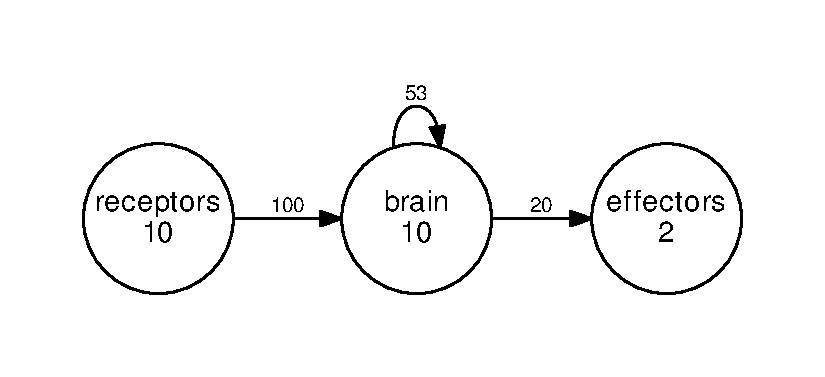
\includegraphics[width=.75\textwidth]{../../example/recnet/recnet-arc}
  \pause
  \lstinputlisting[columns=fullflexible]{../../example/recnet/recnet.arc}    
  \end{center}
  \vfill
\end{frame}

\begin{frame}[fragile]{Code (1)}
  \lstinputlisting[linerange={1-15}]{../../example/recnet/recnet.c}
\end{frame}

\begin{frame}[fragile]{Code (2)}
  \lstinputlisting[linerange={17-32},firstnumber=17]{../../example/recnet/recnet.c}
\end{frame}

\begin{frame}{Results}
  If you run this network, you get an output file with the output of
  ``brain'' cell 0 in response to noise input to the network:
  \begin{center}
    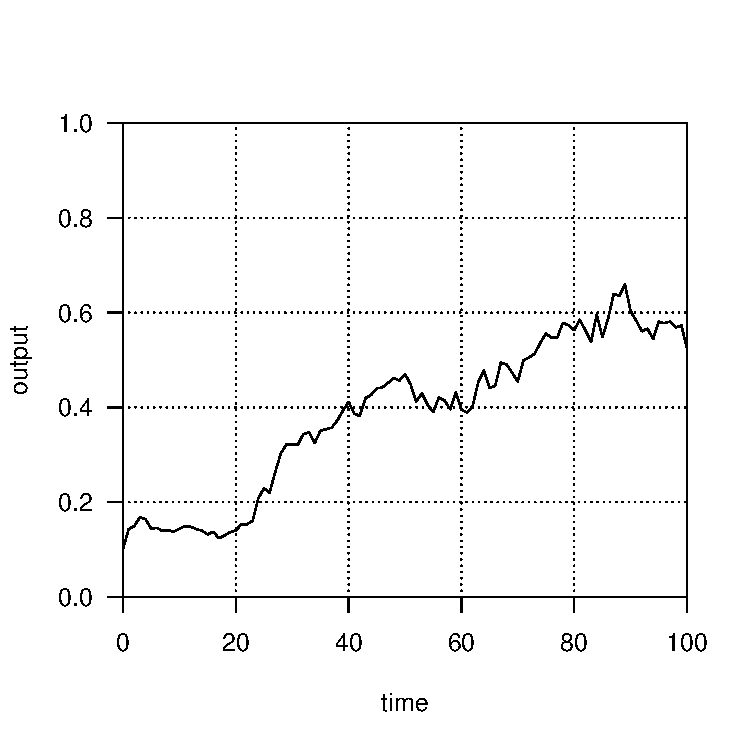
\includegraphics[width=.65\textwidth]{../../example/recnet/recnet}
  \end{center}
  \vfill
\end{frame}

\begin{frame}{What next}
  \begin{itemize}
  \item Is it usable?
  \item Better documentation
  \item Better learning facilities
  \item Visualization has some rough edges
  \item Tests
  \item Feature requests...
  \end{itemize}
\end{frame}
\end{document}
